
\subsection{Comparisons of results}

	Obviously the time of Local search is not comparable to the Exact Method and due to the fact that I set the time for Tabu Search is useless to compare the CPU time between the algorithms used.
	
	Check the differences between the results is much more interesting, figures \ref{fig:comparison} and \ref{fig:fb80-comparison}. We can say that:
	\begin{itemize}
		\item Local Search is the fastest methods.
		\item Tabu Search in almost all cases found the optimal solution or a solution near to optimum;
		\item In general the Tabu Search is better than the Local Search but we need to consider that it requires much more time, 30 seconds versus some milliseconds;
		\item Local Search performs worse for instances with a lot of node.
	\end{itemize}

	\vspace{2cm}
	
	\begin{figure}[bh]
		\centering
		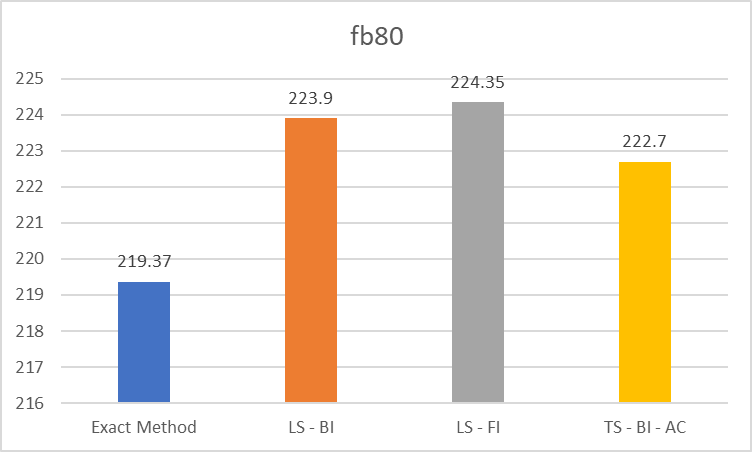
\includegraphics[width=\linewidth]{img/fb80-comparison}
		\caption{Comparison in the fb80 instance. The worse instance for the meta heuristic methods.}
		\label{fig:fb80-comparison}
	\end{figure}
	
	\begin{figure}[h]
		\centering
		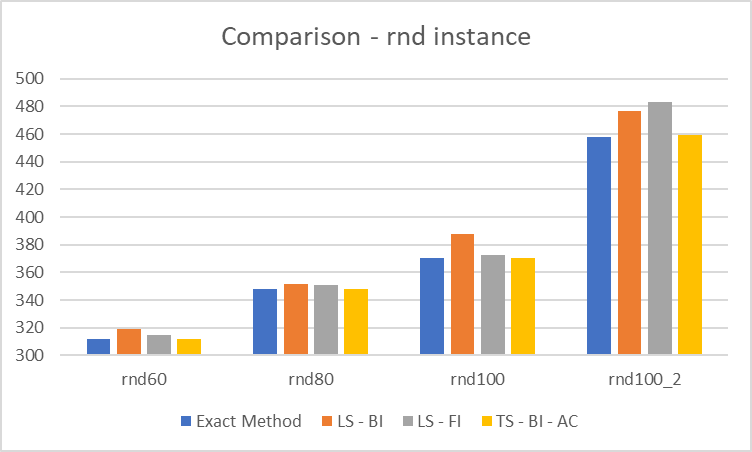
\includegraphics[width=\linewidth]{img/rnd-comparison}

		\vspace{1cm}

		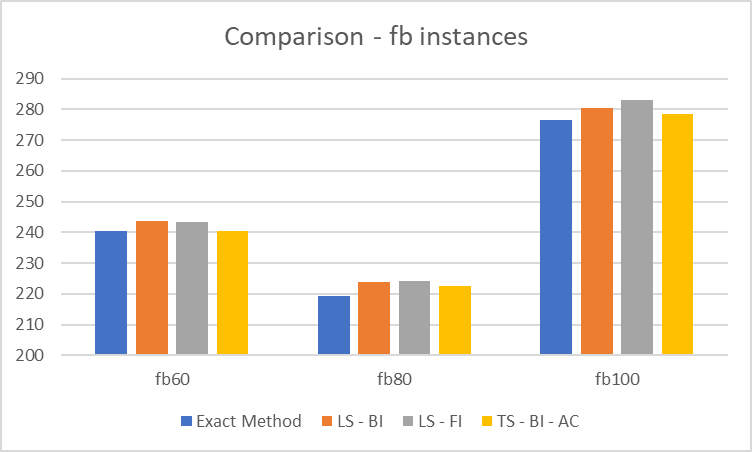
\includegraphics[width=\linewidth]{img/fb-comparison}
		\caption{Comparison of the different methods for rnd and fb instances. \textbf{Note:} in order to mark the difference y-axes doesn't start from 0.}
		\label{fig:comparison}
	\end{figure}

	
	
	